\documentclass[a4paper, 11pt]{article}

%%%%%% 导入包 %%%%%%
%\usepackage{CJKutf8}
\usepackage[unicode]{hyperref}
\usepackage{xcolor}
\usepackage{cite}
\usepackage{indentfirst}
\usepackage{ctex}			%导入 ctex 宏包,添加中文支持
\usepackage{amsmath,amsfonts,amssymb,bm}   %导入数学公式所需宏包
\usepackage{graphicx,hyperref,url}
\usepackage{algorithm, algorithmic}
\usepackage{multirow}
\usepackage{metalogo}	% 非必须

\usepackage{verbatim}


%%%%%% 设置字号 %%%%%%
\newcommand{\chuhao}{\fontsize{42pt}{\baselineskip}\selectfont}
\newcommand{\xiaochuhao}{\fontsize{36pt}{\baselineskip}\selectfont}
\newcommand{\yihao}{\fontsize{28pt}{\baselineskip}\selectfont}
\newcommand{\erhao}{\fontsize{21pt}{\baselineskip}\selectfont}
\newcommand{\xiaoerhao}{\fontsize{18pt}{\baselineskip}\selectfont}
\newcommand{\sanhao}{\fontsize{15.75pt}{\baselineskip}\selectfont}
\newcommand{\sihao}{\fontsize{14pt}{\baselineskip}\selectfont}
\newcommand{\xiaosihao}{\fontsize{12pt}{\baselineskip}\selectfont}
\newcommand{\wuhao}{\fontsize{10.5pt}{\baselineskip}\selectfont}
\newcommand{\xiaowuhao}{\fontsize{9pt}{\baselineskip}\selectfont}
\newcommand{\liuhao}{\fontsize{7.875pt}{\baselineskip}\selectfont}
\newcommand{\qihao}{\fontsize{5.25pt}{\baselineskip}\selectfont}

%%%% 设置 section 属性 %%%%
\makeatletter
\renewcommand\section{\@startsection{section}{1}{\z@}%
{-1.5ex \@plus -.5ex \@minus -.2ex}%
{.5ex \@plus .1ex}%
{\normalfont\sihao\CJKfamily{hei}}}
\makeatother

%%%% 设置 subsection 属性 %%%%
\makeatletter
\renewcommand\subsection{\@startsection{subsection}{1}{\z@}%
{-1.25ex \@plus -.5ex \@minus -.2ex}%
{.4ex \@plus .1ex}%
{\normalfont\xiaosihao\CJKfamily{hei}}}
\makeatother

%%%% 设置 subsubsection 属性 %%%%
\makeatletter
\renewcommand\subsubsection{\@startsection{subsubsection}{1}{\z@}%
{-1ex \@plus -.5ex \@minus -.2ex}%
{.3ex \@plus .1ex}%
{\normalfont\xiaosihao\CJKfamily{hei}}}
\makeatother

%%%% 段落首行缩进两个字 %%%%
\makeatletter
\let\@afterindentfalse\@afterindenttrue
\@afterindenttrue
\makeatother
\setlength{\parindent}{2em}  %中文缩进两个汉字位


%%%% 下面的命令重定义页面边距,使其符合中文刊物习惯 %%%%
\addtolength{\topmargin}{-54pt}
\setlength{\oddsidemargin}{0.63cm}  % 3.17cm - 1 inch
\setlength{\evensidemargin}{\oddsidemargin}
\setlength{\textwidth}{14.66cm}
\setlength{\textheight}{24.00cm}    % 24.62

%%%% 下面的命令设置行间距与段落间距 %%%%
\linespread{1.4}
% \setlength{\parskip}{1ex}
\setlength{\parskip}{0.5\baselineskip}

%%%% 正文开始 %%%%
\begin{document}

%%%% 定理类环境的定义 %%%%
%\newtheorem{example}{例}             % 整体编号
%%\newtheorem{algorithm}{算法}
%\newtheorem{theorem}{定理}[section]  % 按 section 编号
%\newtheorem{definition}{定义}
%\newtheorem{axiom}{公理}
%\newtheorem{property}{性质}
%\newtheorem{proposition}{命题}
%\newtheorem{lemma}{引理}
%\newtheorem{corollary}{推论}
%\newtheorem{remark}{注解}
%\newtheorem{condition}{条件}
%\newtheorem{conclusion}{结论}
%\newtheorem{assumption}{假设}

%%%% 重定义 %%%%
%\renewcommand{\contentsname}{目录}  % 将Contents改为目录
%\renewcommand{\abstractname}{摘要}  % 将Abstract改为摘要
%\renewcommand{\refname}{参考文献}   % 将References改为参考文献
%\renewcommand{\indexname}{索引}
%\renewcommand{\figurename}{图}
%\renewcommand{\tablename}{表}
%\renewcommand{\appendixname}{附录}
%%\renewcommand{\algorithm}{算法}


%%%% 定义标题格式,包括title,author,affiliation,email等 %%%%
\title{生物智能与算法课程报告\\人工鱼群算法}
\author{姓名:罗晓倩\\学号:21721107}
\date{\today}
%%%% 以下部分是正文 %%%%  
\maketitle
\tableofcontents
\newpage
\begin{section}
	{算法背景}提出者:李晓磊等人,2002年。\\提出背景:随着人工智能和人工生命的兴起,出现了一些仿生算法,包括蚁群算法和粒子群算法等。将人工智能的思想应用于问题的寻优,实施一些高级的计算方法。应用动物自治体的模式来定义实体,让他们在问题空间中自主的活动,从而达到解决问题的目的。
\end{section}
\begin{section}
{算法简介}
	\begin{subsection}
	{鱼群模式}
		\begin{subsubsection}
		{视觉}	虚拟人工鱼实体的当前状态为X,Visual为其视野范围,状态$X_v$为其在某时刻视点所在的位置,如果该位置的状态优于当前状态,则考虑向该位置方向前进一步,即到达状态$X_{next}。$
		\begin{figure}[htbp]
			\centering
			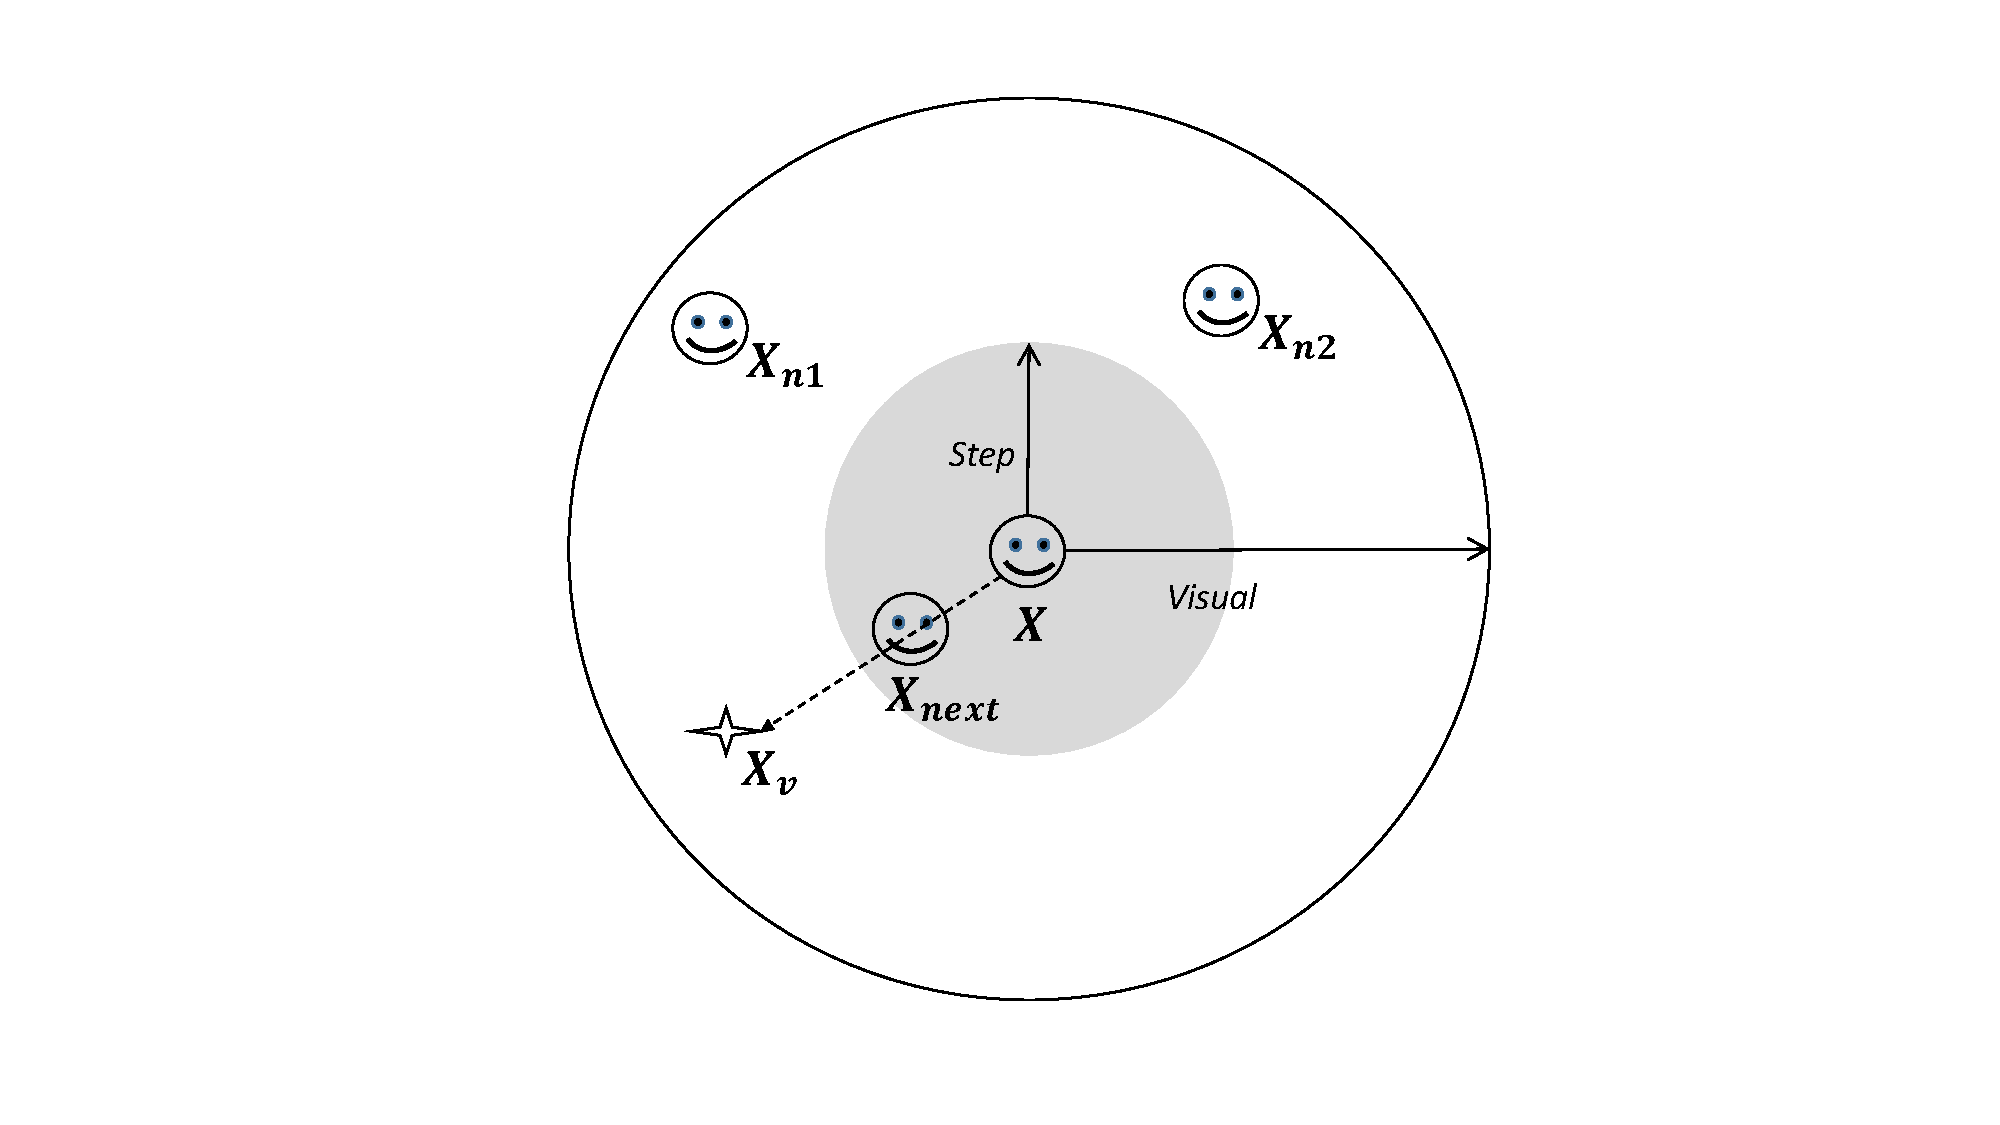
\includegraphics[width=0.5\textwidth]{../pic/fish1.pdf}
			\caption{人工鱼的视野和移动步长}
		\end{figure}
		\end{subsubsection}
		\begin{subsubsection}
		{鱼群行为分析}
		\begin{itemize}
			\item{聚群行为:鱼类进化过程中的一种生存方式,大量或少量的鱼都能聚集成群,进行集体觅食和躲避敌害。}
			\item{追尾行为:当某一条鱼或几条鱼发现食物时,它们附近的鱼会尾随其后快速游过来,进而导致更远处的鱼也尾随过来。}
			\item{随机行为:鱼在水中悠闲的自由游动,基本上是随机的,其视也是为了更大范围地寻觅食物或同伴。}
			\item{觅食行为:生物的基本行为,趋向食物的一种活动。一般可以认定它是同过视觉或味觉来感知水中的食物量或浓度来选择趋向。}
		\end{itemize}
		\end{subsubsection}
		\begin{subsubsection}
		{人工鱼}		人工鱼是真实鱼个体的一个虚拟实体,用来进行问题的分析和说明。\\如图所示,可以将人工鱼看作是一个封装了自身数据星系和一系列行为的一个实体,同过感官来接受环境的刺激信息,并通过控制尾鳍来做出相应的应激活动。\\人工鱼所在的环境主要是问题的解空间和其他人工鱼的状态,它在下一刻的行为取决于目前自身状态和目前环境的状态,并且它还通过自身活动的同时来影响环境,进而影响其他同伴的活动。
		\begin{figure}[htbp]
			\centering
			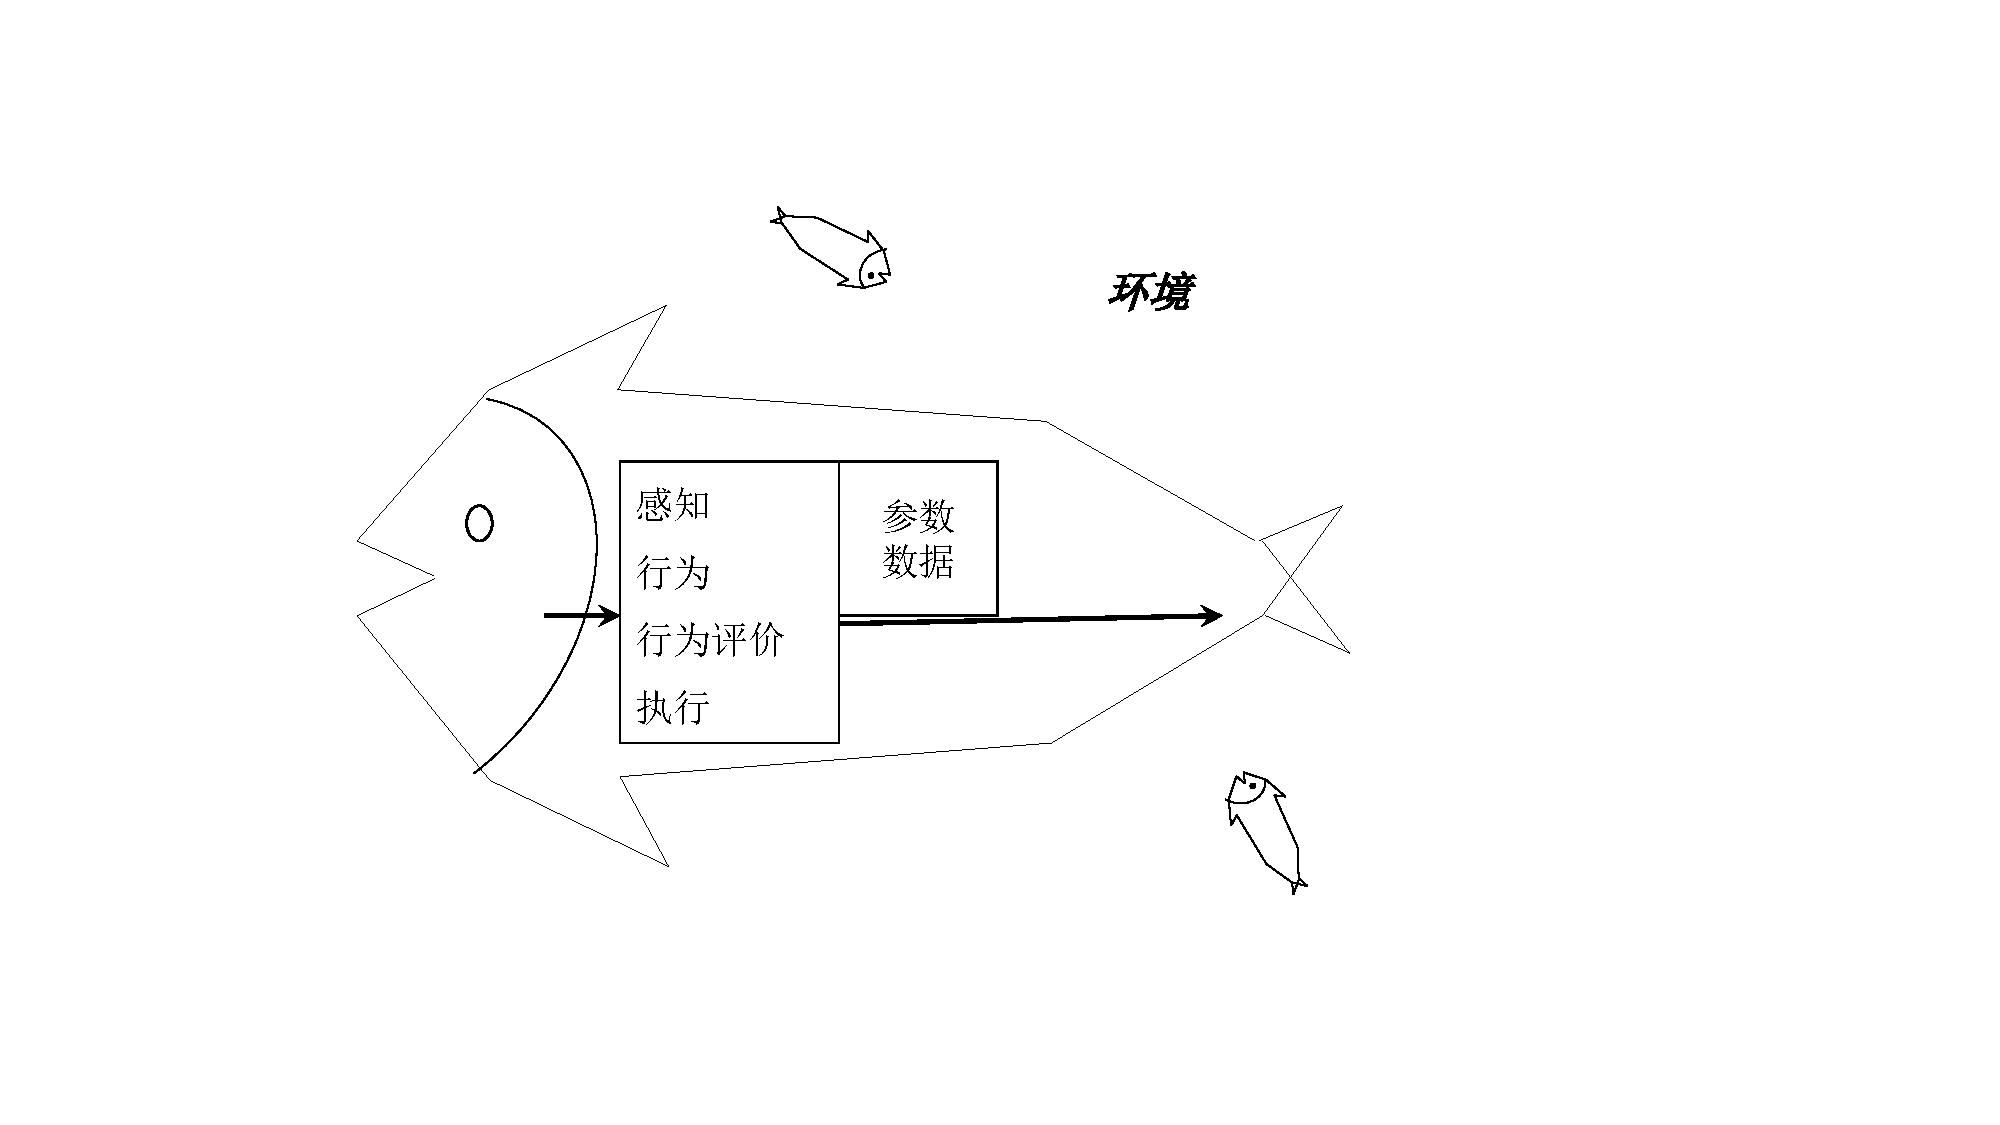
\includegraphics[width=0.9\textwidth]{../pic/fish2.pdf}
			\caption{人工鱼实体}
		\end{figure}
		\end{subsubsection}
		\begin{subsubsection}
			{问题解决}	实际问题的解决是通过自治体在自主的活动过程中以某种形式表现出来的。在一片水域中,鱼生存的数目最多的地方一般就是本水域中富含营养物质最多的地方,依据这一特点来模仿鱼群的觅食等行为,从而实现全局寻优,这就是鱼群算法的基本思想。\\在寻优过程中,通常会有两种方式表现出来:
		\begin{itemize}
			\item{一种形式是通过人工鱼最终的分布情况来确定最优解的分布,通常随着寻优解过程的进展,人工鱼往往会聚集在极值点的周围,而且,全局最优的极值点周围能聚集较多的人工鱼}
			\item{另一种形式是在人工鱼的个体状态之中表现出来的,即在寻优的过程中,跟踪记录最优个体的状态,类似于遗传算法等的方式}
		\end{itemize}
		\end{subsubsection}
	\end{subsection}
	\begin{subsection}
		{人工鱼模型}
		\small{\emph{{class Artificial\underline{\hspace{0.5em}}fish}\\ \indent {\{}\\ \indent Various:\\{\indent\indent{float AF\underline{\hspace{0.5em}}X[n];}\qquad\qquad\qquad\qquad{//AFs position}}\\{\indent\indent{float AF\underline{\hspace{0.5em}}step;}\qquad\qquad\qquad\qquad{//the distance that AF can move for each step}}\\{\indent\indent{float AF\underline{\hspace{0.5em}}visual;}\qquad\qquad\qquad\quad{//the visual distance of AF}}\\{\indent\indent{float try  \underline{\hspace{0.5em}}number}\qquad\qquad\qquad\;{//attempt time in the behacior of prey}}\\{\indent\indent{float delta;}\qquad\qquad\qquad\qquad\quad{//the condition of jamming}}\\{\indent Functions:}\\{\indent\indent{float AF\underline{\hspace{0.5em}}foodconsistence();}\qquad\; {//the food consistence of AFs current position}}\\{\indent\indent{void AF\underline{\hspace{0.5em}}move();}\qquad\qquad\qquad\quad{//AF move to the next position}}\\{\indent\indent{float AF\underline{\hspace{0.5em}}follow();}\qquad\qquad\qquad\ {//the behavior of follow}}\\{\indent\indent{float AF\underline{\hspace{0.5em}}prey();}\qquad\qquad\qquad\quad{//the behavior of prey}}\\{\indent\indent{float AF\underline{\hspace{0.5em}}swarm();}\qquad\qquad\qquad{//the behavior of swarm}}\\{\indent\indent{int AF\underline{\hspace{0.5em}}evaluate();}\qquad\qquad\qquad{//evaluate and select the behavior}}\\{\indent\indent{void AF\underline{\hspace{0.5em}}init();}\qquad\qquad\qquad\quad\ {//to initialize the AF}}\\{\indent\indent{Artificial\underline{\hspace{0.5em}}fish();}}\\{\indent\indent{virtual~Artificial\underline{\hspace{0.5em}}fish;}}\\{\indent \};}}}\\
	Step:人工鱼移动最大步长,{$\delta:$拥挤度因子},Visual:人工鱼感知距离,个体状态:$(x_1,x_2,···,x_n)$,其中$x_i$为欲寻优的变量,Y=f(X)表示当前所在位置食物浓度,人工鱼个体之间的距离:$d_{i,j}=|X_i-X_j|$
	\end{subsection}

	\begin{subsection}
		{行为描述}
%		觅食行为
%		\flushleft
%		\scriptsize{\emph{float Aritificial\underline{\hspace{0.5em}}fish::AF\underline{\hspace{0.5em}}prey()\\{\{}\\{\hspace{2em} for($i=0;i<try\underline{\hspace{0.5em}}number;i++)$}\\{\hspace{2em} \{}\\{\hspace{4em}  $X_j=X_i+Rand()·Visual;$}\\{\hspace{4em}   if $(Y_i<Y_j)$}\\{\hspace{6em}  $X_{i|next}=X_i+Rand()·Step·(X_j-X_i)/\lVert X_j-X_i\rVert;$}\\{\hspace{4em}  else}\\{\hspace{6em}    $X_{i|next}=X_i+Rand()·Step;$}\\{\hspace{2em} \}}\\{ return $AF\underline{\hspace{0.5em}}foodconsistence(X_{i|next});$} \\{\}} }}	\\
		\small{觅食行为}
			\flushleft\scriptsize{\emph{float Aritificial\underline{\hspace{0.5em}}fish::AF\underline{\hspace{0.5em}}prey()\\{\{}\\{\qquad for($i=0;i<try\underline{\hspace{0.5em}}number;i++)$}\\{\qquad\{}\\{\qquad\qquad$X_j=X_i+Rand()·Visual;$}\\{\qquad\qquad if $(Y_i<Y_j)$}\\{\qquad\qquad\qquad $X_{i|next}=X_i+Rand()·Step·(X_j-X_i)/\lVert X_j-X_i\rVert;$}\\{\qquad\qquad else}\\{\qquad\qquad\qquad $X_{i|next}=X_i+Rand()·Step;$}\\{\qquad\}}\\{ return $AF\underline{\hspace{0.5em}}foodconsistence(X_{i|next});$} \\{\}} }}\\
		\small{聚群行为}\vspace{3ex}
			\flushleft\scriptsize{\emph{float Aritificial\underline{\hspace{0.5em}}fish::AF\underline{\hspace{0.5em}}swarm() \\ {\{} \\ {\qquad $n_f=0;X_c=0$} \\ {\qquad for($j=0;i<friend\underline{\hspace{0.5em}}number;j++)$} \\ {\qquad\qquad $if(d_{i.j}<Visual) \{ n_f++;X_c+=X_j;\}$} \\ {\qquad $X_c=X_c/n_f;$}\\{\qquad $if (Y_c/n_f>\delta Y_i)$}\\{\qquad\qquad $X_{i|next}=X_i+Rand()·Step·(X_c-X_i)/\lVert X_c-X_i\rVert;$}\\{\qquad else}\\{\qquad\qquad AF\underline{\hspace{0.5em}}prey();}\\{ return $AF\underline{\hspace{0.5em}}foodconsistence(X_{i|next});$} \\{\}} }}\\
		\small{追尾行为}\vspace{3ex}\\
			\flushleft\scriptsize{\emph{float Aritificial\underline{\hspace{0.5em}}fish::AF\underline{\hspace{0.5em}}follow() \\ {\{} \\ {\qquad $Y_max=-\infty;$} \\ {\qquad for($j=0;i<friend\underline{\hspace{0.5em}}number;j++)$} \\ {\qquad\qquad $if(d_{i,j}<Visual \&\& Y_j>Y_max)$} \\ {\qquad\qquad\qquad $\{ Y_max=Y_j; X_max=X_j; \}$ }\\{\qquad $n_f=0$}\\{\qquad for($j=0;i<friend\underline{\hspace{0.5em}}number;j++)$}\\{\qquad\qquad $if(d_{max,j}<Visual) \{ n_f++;\} $}\\{\qquad $if (Y_max/n_f>\delta Y_i)$}\\{\qquad\qquad $X_{i|next}=X_i+Rand()·Step·(X_max-X_i)/\lVert X_max-X_i\rVert;$}\\{\qquad else}\\{\qquad\qquad AF\underline{\hspace{0.5em}}prey();}\\{ return $AF\underline{\hspace{0.5em}}foodconsistence(X_{i|next});$} \\{\}} }}\\
		\small{随机行为}\vspace{3ex}\\
		\vspace{6ex}随机行为的实现即在视野中随机选择一个状态,然后向该方向移动,实际上就是觅食行为的一个缺省行为。
	\end{subsection}
	\begin{subsection}{算法描述}
	每个人工鱼探索它的环境状况(包括目标函数的变化情况和伙伴的变化情况),从而选择一种行为\\最终,人工鱼集结在几个局部极值的周围\\一般情况下,在讨论求极大问题时,拥有较大的$AF\underline{\hspace{0.5em}}foodconsistence$值的人工鱼一般处于值较大的极值域周围\\这有助于获取全局极值域,而值较大的极值区域周围一般能集结较多的人工鱼,这有助于判断并获取全局极值。
		\begin{figure}[htbp]
			\centering
			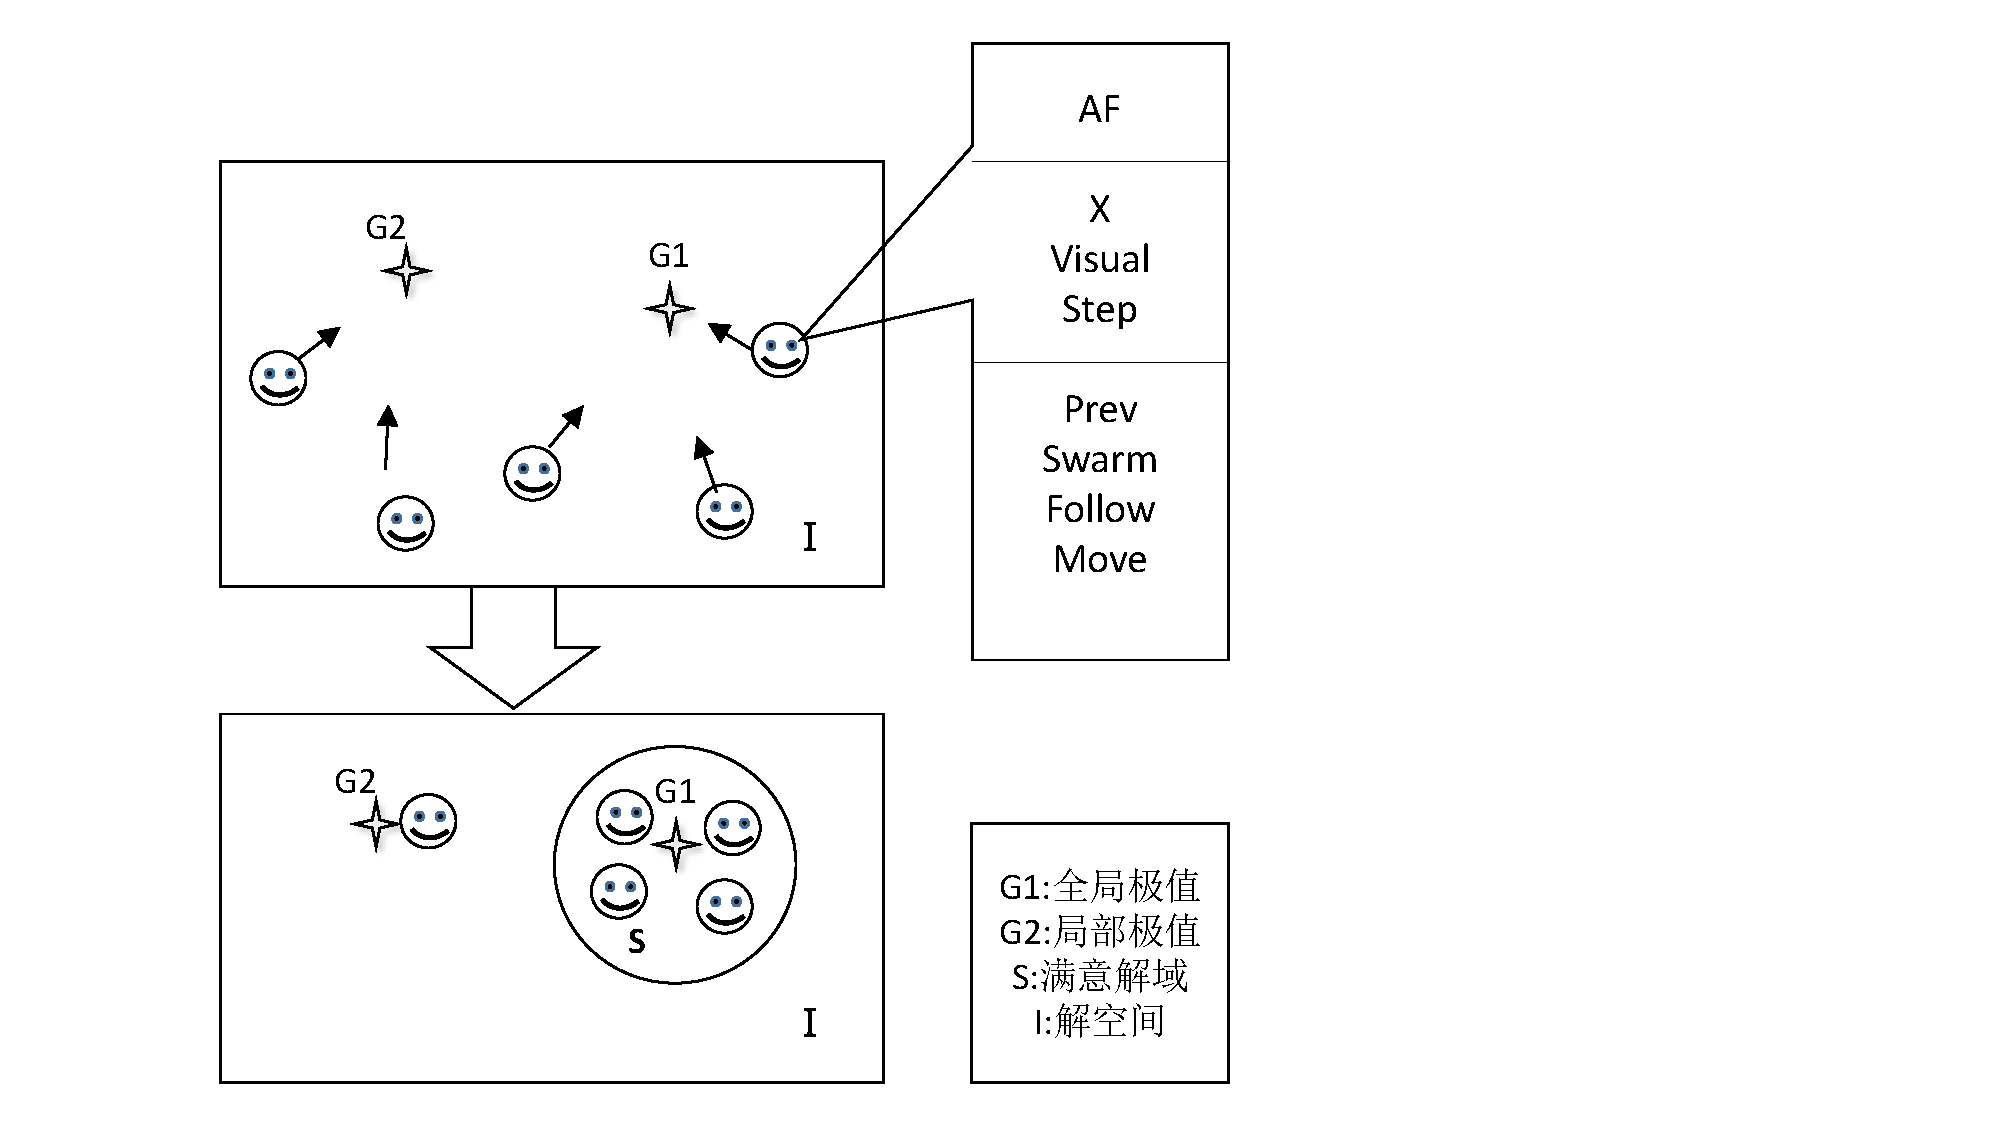
\includegraphics[width=0.5\textwidth]{../pic/fish3.pdf}
			\caption{算法示意图}
		\end{figure}
	\end{subsection}
\end{section}
\begin{section}{算法实现}
	\begin{algorithm}[H]
	\caption{AFA算法}\label{fish_alg}
	\algsetup{linenosize=\tiny} \scriptsize
		\begin{algorithmic}
			\STATE{$::AF\underline{\hspace{0.5em}}init();$}
			\WHILE{the resulr is satisfied}
				\STATE{\textbf{switch}$(::AF\underline{\hspace{0.5em}}evaluat())$}	
				\STATE{\textbf{\quad case}\quad value1:}
				\STATE{$\qquad ::AF\underline{\hspace{0.5em}}follow();$}
				\STATE{\textbf{\quad case}\quad value1:}
				\STATE{\qquad $::AF\underline{\hspace{0.5em}}swarm();$}
				\STATE{\quad \textbf{default$:$}}
				\STATE{\qquad $::AF\underline{\hspace{0.5em}}prey();$}
				\STATE{\textbf{end switch}}			
				\STATE{$AF\underline{\hspace{0.5em}}move();$}
				\STATE{$get\underline{\hspace{0.5em}}result();$}
			\ENDWHILE
			
		\end{algorithmic}
	\end{algorithm}
	\begin{subsection}{各参数对计算时间的影响}
	\begin{figure}[htbp]
		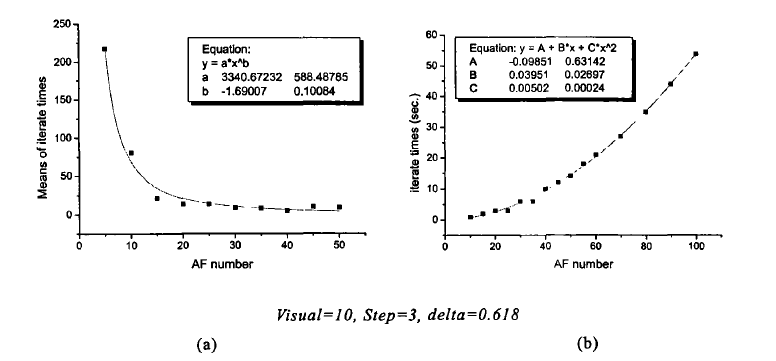
\includegraphics[width=1.0\textwidth]{../pic/fish6.png}
	\end{figure}
	\begin{figure}[htbp]
		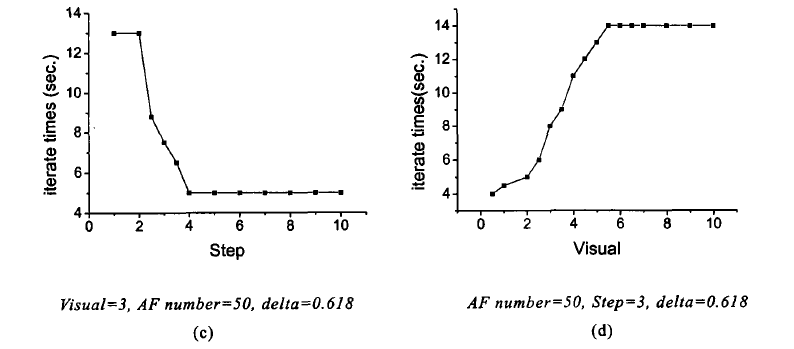
\includegraphics[width=1.0\textwidth]{../pic/fish7.png}
	\end{figure}
	\begin{figure}[htbp]
		\centering
		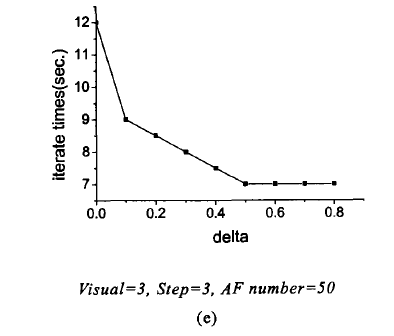
\includegraphics[width=0.5\textwidth]{../pic/fish8.png}
	\end{figure}
	\end{subsection}
	\begin{subsection}{算法特点}
	\begin{itemize}
		\item{算法只需要比较目标函数值,对目标函数的性质要求不高}
		\item{算法对初值的要求不高,初值随机产生或设定为固定值均可以}
		\item{算法对参数设定的要求不高,有较大的容许范围}
		\item{算法具备并行处理的能力,寻优速度较快}
		\item{算法具备全局寻优的能力}
	\end{itemize}
	\end{subsection}
\end{section}
\begin{section}{算法应用}
\begin{subsection}{旅行商问题}
	数据来源:http://www.uni-heidelberg.de/iwr/comopt/software/TSPLIB95/;
	\begin{figure}[htbp]
		\centering
		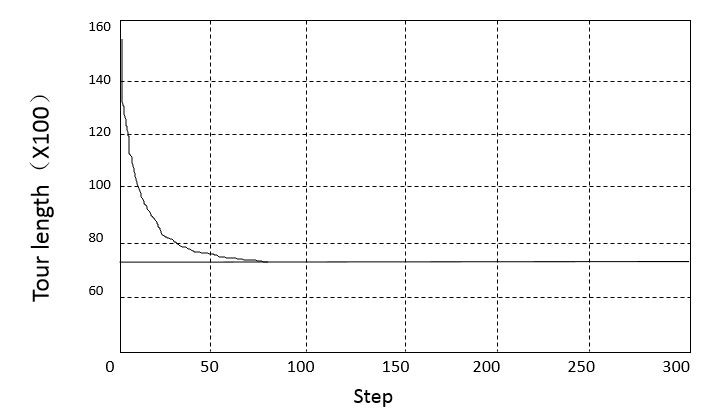
\includegraphics[width=0.8\textwidth]{../pic/fish4.png}
		\caption{Ulysses 22 城市TSP问题的寻优曲线}
	\end{figure}
	\begin{figure}[htbp]
		\centering
		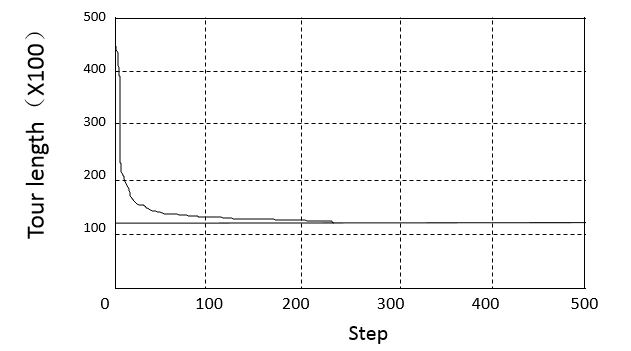
\includegraphics[width=0.8\textwidth]{../pic/fish5.png}
		\caption{Att48 城市TSP问题的寻优曲线}
	\end{figure}
在仿真实验中,为了反映算法对组合优化问题的解决能力,没有针对TSP问题的特点添加任何的启发规则,完全依靠人工鱼群算法对解空间的寻优能力,可见,人工鱼群算法具有较快的收敛速度,但是随着问题规模的扩大,其寻优的精度会有所降低,这是有待改进的地方。
\end{subsection}


	\begin{thebibliography}{123} 
	\bibitem{fish_bib1} 李晓磊,邵之江,钱积新.一种基于动物自治体的寻优模式:鱼群算法[J].系统工程理论与实践,2002,22(11):32 -38.
	\bibitem{fish_bib2} 李晓磊.一种新到的智能优化方法———人工鱼群算法[D].杭州:浙江大学,2003.
	\bibitem{fish_bib3}李晓磊,钱积新.基于分解协调的人工鱼群优化算法研究[J].电路与系统学报,2003,8(1) : 1 -6.
	\end{thebibliography}

\end{section}

\end{document}